\chapter{Prototypische Implementierung}
\label{chap:impl}
Dieses Kapitel widmet sich der prototypischen Implementierung der im vorigen Kapitel vorgestellen Konzeption, die als Vorgabe in C++ entwickelt werden muss. Anhand des UML-Klassendiagrammes in \Fref[plain]{fig:uml} wird der grobe Aufbau gezeigt. Als nächster Punkt wird die Abstraktion des Netwerkes erklärt. Danach wird -- ausgehend von der Applikation -- die Implementierung des Publish/Subscribe-Systems erläutert. Angewandte Techniken wie \ac{tmp} oder \emph{policy based}-Design werden im Anhang dieser Arbeit beschrieben. Sie werden benötigt um den zusätzlichen Verwaltungsaufwand zur Laufzeit durch geschickte Anwendung des zur Übersetzungszeit vorhandenen Wissens zu minimieren. Das nutzbare Wissen umfasst zum Beispiel die Typen der Events, die zur Optimierung ausgewählten Strategien und deren Besonderheiten.

\Fref{fig:uml} stellt ein vereinfachtes Klassenmodell des Frameworks dar. Nicht abgebildet sind Datentypen zum Austausch mit den Netzwerkkomponenten oder sonstige Hilfsstrukturen. \emph{P2PInterface} ist eine abstrakte Basisklasse und repräsentiert die in \cite{Dabek2003Towards} beschrieben KBR-API. Aktuell wird diese vom \emph{ChimeraWrapper} implementiert, der über den \emph{ChimeraWrapperImpl} mit dem Netzwerk Chimera spricht. Hier wurde das ``PIMPL''-Pattern angewandt, mit dem die eigentliche Implementierung versteckt werden kann \cite{Alexandrescu2001Modern}. Zur Vereinfachung werden sämtliche Identifikationsdaten, zum Beispiel die Adresse eines Knotens, des Netzwerkes als \emph{std::string} repräsentiert. Dies entbindet den Entwickler der Implementierung weiterer Wrapperklassen. Sollte ein std::string nicht ausreichen um die nötige Information bereitzustellen muss eine Hashmap als weitere Indirektion eingebunden werden. Zur Nachrichtenübertragung wird der Datentyp \emph{std::vector<char>} bereitgestellt, also die objektorientierte Version eines \emph{char*}. Dies bietet zusätzlichen Schutz gegen Bufferüberlauf oder ähnliche Probleme.\\
Für weitere Netzwerke können auf einfache Art und Weise Wrapperklassen geschrieben und eingebunden werden.

\begin{figure}[htbp]
\centering
\resizebox{\textwidth}{!}{%
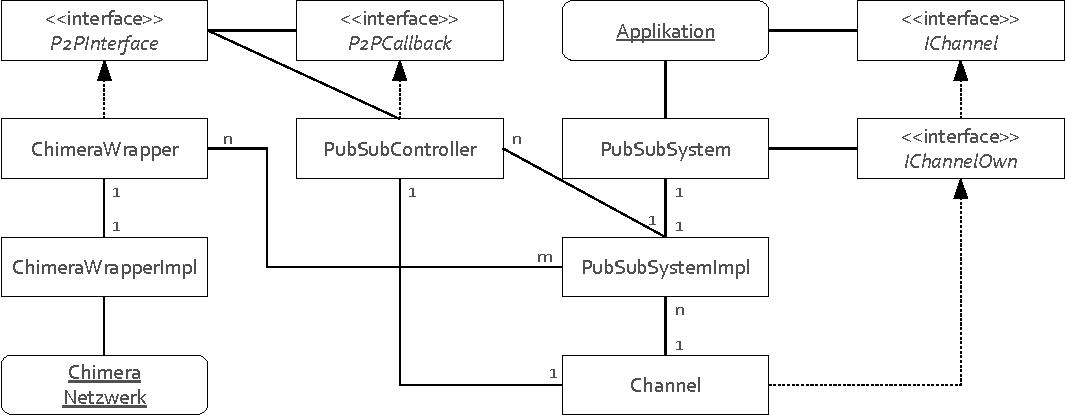
\includegraphics{grafics/uml.pdf}}
\caption{vereinfachtes Klassendiagramm des Frameworks}
\label{fig:uml}
\end{figure}

Die \emph{Applikation} greift auf das Publish/Subscribe-System über den Singleton \emph{PubSubSytem} zu. Beiden ist der optimierte \emph{Channel} nur über die abstrakten Basisklassen \emph{IChannel} beziehungsweise \emph{IChannelOwn} zugänglich. Diese bieten lediglich die drei üblichen Methoden für Publish/Subscribe-Systeme\footnote{subscribe, unsubscribe und publish} an. Dadurch ist die Komplexität der Klasse Channel verdeckt. Der Channel ist eine mit policy-based Design erstellte Templateklassen\footnote{siehe \Fref{chap:impl_tmp} im Anhang zur Erklärung}. Die verschiedenen Strategien -- in \Fref{fig:uml} ebenfalls nicht dargestellt -- werden dem Channel als Policies übergeben. Durch \ac{tmp} ist es zudem möglich jeden Channel auf die gewählten Policies abzustimmen. Weiterhin wird für jeden Channel ein optimierten Header erzeugt, dessen Größe an Nutzlast von den gewählten Policies abhängig ist. Durch diese Maßnahmen wird der Overhead zur Laufzeit stark reduziert. 

Die Klasse \emph{PubSubController} implementiert das Interface \emph{P2PCallback} und kann sich somit für die Callbacks des Netzwerkes registrieren. Der PubSubController ist die Schnittstelle des Publish/Subscribe-Systems mit dem \ac{p2p}-Netzwerk und bietet die benötigte Funktionalität für die Klasse Channel. Zudem werden die ankommenden Nachrichten in deliver über eine Queue und einen Dispatch-Thread an die einzelnen Kanäle verteilt. \emph{PubSubSystemImpl} kennt die verschiedenen Netzwerkwrapper (in \Fref{fig:uml} ist dies ChimeraWrapper) und instantiiert für jedes genutztes Netzwerk einen PubSubController und übergibt diesen an jeden einzelnen Channel. Mit verschiedene Instanzen des PubSubControllers können somit auch verschiedene Netzwerke angesprochen werden und entsprechend der Optimierung für verschiedene Channel eingesetzt werden. Innerhalb der Klasse PubSubSystemImpl werden Instanzten der optimierten Kanäle als Klassenvariablen verwaltet.

Im Optimierungsschritt müssen daher folgende Klassen generiert und angepasst werden:
\begin{description}
\item[ChannelList.h] In dieser Datei ist eine Liste der vorhandenen Kanäle als ``enum'' abgelegt. Diese Einträge müssen bei der Kommunikation mit dem PubSubSytem genutzt werden um den entsprechenden Kanal zu wählen.
\item[PubSubSystemImpl.h] Diese Klasse muss komplett generiert werden. Sie hat Zugriff auf alle zur Optimierung genutzten Strategien und den daraus erzeugten Instanzen der Templateklasse Channel. Zudem können hier die verschiedenen Netzwerke mit den verschiedenen Kanälen durch die Klasse PubSubController verbunden werden. 
\item[PubSubSytem.cpp] Die Klasse PubSubSystem greift direkt auf die in PubSubSystemImpl definierten Kanäle (als IChannelOwn*) zu. Da diese erst im Optimierungschritt bekannt sind, muss dies ebenfalls generiert werden, soll ein Abgleich beziehungsweise eine Suche zur Laufzeit vermieden werden.
\end{description}

\lstinputlisting[caption={Zugriff auf M$^2$etis aus Benutzersicht}, label=lst:pubsub_usage]{listings/pubsub_usage.cpp}


